
%% bare_jrnl.tex
%% V1.4
%% 2012/12/27
%% by Michael Shell
%% see http://www.michaelshell.org/
%% for current contact information.
%%
%% This is a skeleton file demonstrating the use of IEEEtran.cls
%% (requires IEEEtran.cls version 1.8 or later) with an IEEE journal paper.
%%
%% Support sites:
%% http://www.michaelshell.org/tex/ieeetran/
%% http://www.ctan.org/tex-archive/macros/latex/contrib/IEEEtran/
%% and
%% http://www.ieee.org/



% *** Authors should verify (and, if needed, correct) their LaTeX system  ***
% *** with the testflow diagnostic prior to trusting their LaTeX platform ***
% *** with production work. IEEE's font choices can trigger bugs that do  ***
% *** not appear when using other class files.                            ***
% The testflow support page is at:
% http://www.michaelshell.org/tex/testflow/


%%*************************************************************************
%% Legal Notice:
%% This code is offered as-is without any warranty either expressed or
%% implied; without even the implied warranty of MERCHANTABILITY or
%% FITNESS FOR A PARTICULAR PURPOSE! 
%% User assumes all risk.
%% In no event shall IEEE or any contributor to this code be liable for
%% any damages or losses, including, but not limited to, incidental,
%% consequential, or any other damages, resulting from the use or misuse
%% of any information contained here.
%%
%% All comments are the opinions of their respective authors and are not
%% necessarily endorsed by the IEEE.
%%
%% This work is distributed under the LaTeX Project Public License (LPPL)
%% ( http://www.latex-project.org/ ) version 1.3, and may be freely used,
%% distributed and modified. A copy of the LPPL, version 1.3, is included
%% in the base LaTeX documentation of all distributions of LaTeX released
%% 2003/12/01 or later.
%% Retain all contribution notices and credits.
%% ** Modified files should be clearly indicated as such, including  **
%% ** renaming them and changing author support contact information. **
%%
%% File list of work: IEEEtran.cls, IEEEtran_HOWTO.pdf, bare_adv.tex,
%%                    bare_conf.tex, bare_jrnl.tex, bare_jrnl_compsoc.tex,
%%                    bare_jrnl_transmag.tex
%%*************************************************************************

% Note that the a4paper option is mainly intended so that authors in
% countries using A4 can easily print to A4 and see how their papers will
% look in print - the typesetting of the document will not typically be
% affected with changes in paper size (but the bottom and side margins will).
% Use the testflow package mentioned above to verify correct handling of
% both paper sizes by the user's LaTeX system.
%
% Also note that the "draftcls" or "draftclsnofoot", not "draft", option
% should be used if it is desired that the figures are to be displayed in
% draft mode.
%
\documentclass[conference]{IEEEtran}
%
% If IEEEtran.cls has not been installed into the LaTeX system files,
% manually specify the path to it like:
% \documentclass[journal]{../sty/IEEEtran}





% Some very useful LaTeX packages include:
% (uncomment the ones you want to load)


% *** MISC UTILITY PACKAGES ***
%
%\usepackage{ifpdf}
% Heiko Oberdiek's ifpdf.sty is very useful if you need conditional
% compilation based on whether the output is pdf or dvi.
% usage:
% \ifpdf
%   % pdf code
% \else
%   % dvi code
% \fi
% The latest version of ifpdf.sty can be obtained from:
% http://www.ctan.org/tex-archive/macros/latex/contrib/oberdiek/
% Also, note that IEEEtran.cls V1.7 and later provides a builtin
% \ifCLASSINFOpdf conditional that works the same way.
% When switching from latex to pdflatex and vice-versa, the compiler may
% have to be run twice to clear warning/error messages.





% *** CITATION PACKAGES ***
%
\usepackage{cite}
% cite.sty was written by Donald Arseneau
% V1.6 and later of IEEEtran pre-defines the format of the cite.sty package
% \cite{} output to follow that of IEEE. Loading the cite package will
% result in citation numbers being automatically sorted and properly
% "compressed/ranged". e.g., [1], [9], [2], [7], [5], [6] without using
% cite.sty will become [1], [2], [5]--[7], [9] using cite.sty. cite.sty's
% \cite will automatically add leading space, if needed. Use cite.sty's
% noadjust option (cite.sty V3.8 and later) if you want to turn this off
% such as if a citation ever needs to be enclosed in parenthesis.
% cite.sty is already installed on most LaTeX systems. Be sure and use
% version 4.0 (2003-05-27) and later if using hyperref.sty. cite.sty does
% not currently provide for hyperlinked citations.
% The latest version can be obtained at:
% http://www.ctan.org/tex-archive/macros/latex/contrib/cite/
% The documentation is contained in the cite.sty file itself.






% *** GRAPHICS RELATED PACKAGES ***
%
%\ifCLASSINFOpdf
  % \usepackage[pdftex]{graphicx}
  % declare the path(s) where your graphic files are
  % \graphicspath{{../pdf/}{../jpeg/}}
  % and their extensions so you won't have to specify these with
  % every instance of \includegraphics
  % \DeclareGraphicsExtensions{.pdf,.jpeg,.png}
%\else
  % or other class option (dvipsone, dvipdf, if not using dvips). graphicx
  % will default to the driver specified in the system graphics.cfg if no
  % driver is specified.
\usepackage{graphicx}
  % declare the path(s) where your graphic files are
  % \graphicspath{{../eps/}}
  % and their extensions so you won't have to specify these with
  % every instance of \includegraphics
  % \DeclareGraphicsExtensions{.eps}
%\fi
% graphicx was written by David Carlisle and Sebastian Rahtz. It is
% required if you want graphics, photos, etc. graphicx.sty is already
% installed on most LaTeX systems. The latest version and documentation
% can be obtained at: 
% http://www.ctan.org/tex-archive/macros/latex/required/graphics/
% Another good source of documentation is "Using Imported Graphics in
% LaTeX2e" by Keith Reckdahl which can be found at:
% http://www.ctan.org/tex-archive/info/epslatex/
%
% latex, and pdflatex in dvi mode, support graphics in encapsulated
% postscript (.eps) format. pdflatex in pdf mode supports graphics
% in .pdf, .jpeg, .png and .mps (metapost) formats. Users should ensure
% that all non-photo figures use a vector format (.eps, .pdf, .mps) and
% not a bitmapped formats (.jpeg, .png). IEEE frowns on bitmapped formats
% which can result in "jaggedy"/blurry rendering of lines and letters as
% well as large increases in file sizes.
%
% You can find documentation about the pdfTeX application at:
% http://www.tug.org/applications/pdftex





% *** MATH PACKAGES ***
%
\usepackage[cmex10]{amsmath}
% A popular package from the American Mathematical Society that provides
% many useful and powerful commands for dealing with mathematics. If using
% it, be sure to load this package with the cmex10 option to ensure that
% only type 1 fonts will utilized at all point sizes. Without this option,
% it is possible that some math symbols, particularly those within
% footnotes, will be rendered in bitmap form which will result in a
% document that can not be IEEE Xplore compliant!
%
% Also, note that the amsmath package sets \interdisplaylinepenalty to 10000
% thus preventing page breaks from occurring within multiline equations. Use:
%\interdisplaylinepenalty=2500
% after loading amsmath to restore such page breaks as IEEEtran.cls normally
% does. amsmath.sty is already installed on most LaTeX systems. The latest
% version and documentation can be obtained at:
% http://www.ctan.org/tex-archive/macros/latex/required/amslatex/math/





% *** SPECIALIZED LIST PACKAGES ***
%
%\usepackage{algorithmic}
% algorithmic.sty was written by Peter Williams and Rogerio Brito.
% This package provides an algorithmic environment fo describing algorithms.
% You can use the algorithmic environment in-text or within a figure
% environment to provide for a floating algorithm. Do NOT use the algorithm
% floating environment provided by algorithm.sty (by the same authors) or
% algorithm2e.sty (by Christophe Fiorio) as IEEE does not use dedicated
% algorithm float types and packages that provide these will not provide
% correct IEEE style captions. The latest version and documentation of
% algorithmic.sty can be obtained at:
% http://www.ctan.org/tex-archive/macros/latex/contrib/algorithms/
% There is also a support site at:
% http://algorithms.berlios.de/index.html
% Also of interest may be the (relatively newer and more customizable)
% algorithmicx.sty package by Szasz Janos:
% http://www.ctan.org/tex-archive/macros/latex/contrib/algorithmicx/




% *** ALIGNMENT PACKAGES ***
%
\usepackage{tabularx}
\usepackage{array}
\newcolumntype{L}{>{\raggedright\arraybackslash}X}%
% Frank Mittelbach's and David Carlisle's array.sty patches and improves
% the standard LaTeX2e array and tabular environments to provide better
% appearance and additional user controls. As the default LaTeX2e table
% generation code is lacking to the point of almost being broken with
% respect to the quality of the end results, all users are strongly
% advised to use an enhanced (at the very least that provided by array.sty)
% set of table tools. array.sty is already installed on most systems. The
% latest version and documentation can be obtained at:
% http://www.ctan.org/tex-archive/macros/latex/required/tools/


% IEEEtran contains the IEEEeqnarray family of commands that can be used to
% generate multiline equations as well as matrices, tables, etc., of high
% quality.




% *** SUBFIGURE PACKAGES ***
%\ifCLASSOPTIONcompsoc
%  \usepackage[caption=false,font=normalsize,labelfont=sf,textfont=sf]{subfig}
%\else
%  \usepackage[caption=false,font=footnotesize]{subfig}
%\fi
% subfig.sty, written by Steven Douglas Cochran, is the modern replacement
% for subfigure.sty, the latter of which is no longer maintained and is
% incompatible with some LaTeX packages including fixltx2e. However,
% subfig.sty requires and automatically loads Axel Sommerfeldt's caption.sty
% which will override IEEEtran.cls' handling of captions and this will result
% in non-IEEE style figure/table captions. To prevent this problem, be sure
% and invoke subfig.sty's "caption=false" package option (available since
% subfig.sty version 1.3, 2005/06/28) as this is will preserve IEEEtran.cls
% handling of captions.
% Note that the Computer Society format requires a larger sans serif font
% than the serif footnote size font used in traditional IEEE formatting
% and thus the need to invoke different subfig.sty package options depending
% on whether compsoc mode has been enabled.
%
% The latest version and documentation of subfig.sty can be obtained at:
% http://www.ctan.org/tex-archive/macros/latex/contrib/subfig/




% *** FLOAT PACKAGES ***
%
\usepackage{fixltx2e}
% fixltx2e, the successor to the earlier fix2col.sty, was written by
% Frank Mittelbach and David Carlisle. This package corrects a few problems
% in the LaTeX2e kernel, the most notable of which is that in current
% LaTeX2e releases, the ordering of single and double column floats is not
% guaranteed to be preserved. Thus, an unpatched LaTeX2e can allow a
% single column figure to be placed prior to an earlier double column
% figure. The latest version and documentation can be found at:
% http://www.ctan.org/tex-archive/macros/latex/base/


%\usepackage{stfloats}
% stfloats.sty was written by Sigitas Tolusis. This package gives LaTeX2e
% the ability to do double column floats at the bottom of the page as well
% as the top. (e.g., "\begin{figure*}[!b]" is not normally possible in
% LaTeX2e). It also provides a command:
%\fnbelowfloat
% to enable the placement of footnotes below bottom floats (the standard
% LaTeX2e kernel puts them above bottom floats). This is an invasive package
% which rewrites many portions of the LaTeX2e float routines. It may not work
% with other packages that modify the LaTeX2e float routines. The latest
% version and documentation can be obtained at:
% http://www.ctan.org/tex-archive/macros/latex/contrib/sttools/
% Do not use the stfloats baselinefloat ability as IEEE does not allow
% \baselineskip to stretch. Authors submitting work to the IEEE should note
% that IEEE rarely uses double column equations and that authors should try
% to avoid such use. Do not be tempted to use the cuted.sty or midfloat.sty
% packages (also by Sigitas Tolusis) as IEEE does not format its papers in
% such ways.
% Do not attempt to use stfloats with fixltx2e as they are incompatible.
% Instead, use Morten Hogholm'a dblfloatfix which combines the features
% of both fixltx2e and stfloats:
%
% \usepackage{dblfloatfix}
% The latest version can be found at:
% http://www.ctan.org/tex-archive/macros/latex/contrib/dblfloatfix/




%\ifCLASSOPTIONcaptionsoff
%  \usepackage[nomarkers]{endfloat}
% \let\MYoriglatexcaption\caption
% \renewcommand{\caption}[2][\relax]{\MYoriglatexcaption[#2]{#2}}
%\fi
% endfloat.sty was written by James Darrell McCauley, Jeff Goldberg and 
% Axel Sommerfeldt. This package may be useful when used in conjunction with 
% IEEEtran.cls'  captionsoff option. Some IEEE journals/societies require that
% submissions have lists of figures/tables at the end of the paper and that
% figures/tables without any captions are placed on a page by themselves at
% the end of the document. If needed, the draftcls IEEEtran class option or
% \CLASSINPUTbaselinestretch interface can be used to increase the line
% spacing as well. Be sure and use the nomarkers option of endfloat to
% prevent endfloat from "marking" where the figures would have been placed
% in the text. The two hack lines of code above are a slight modification of
% that suggested by in the endfloat docs (section 8.4.1) to ensure that
% the full captions always appear in the list of figures/tables - even if
% the user used the short optional argument of \caption[]{}.
% IEEE papers do not typically make use of \caption[]'s optional argument,
% so this should not be an issue. A similar trick can be used to disable
% captions of packages such as subfig.sty that lack options to turn off
% the subcaptions:
% For subfig.sty:
% \let\MYorigsubfloat\subfloat
% \renewcommand{\subfloat}[2][\relax]{\MYorigsubfloat[]{#2}}
% However, the above trick will not work if both optional arguments of
% the \subfloat command are used. Furthermore, there needs to be a
% description of each subfigure *somewhere* and endfloat does not add
% subfigure captions to its list of figures. Thus, the best approach is to
% avoid the use of subfigure captions (many IEEE journals avoid them anyway)
% and instead reference/explain all the subfigures within the main caption.
% The latest version of endfloat.sty and its documentation can obtained at:
% http://www.ctan.org/tex-archive/macros/latex/contrib/endfloat/
%
% The IEEEtran \ifCLASSOPTIONcaptionsoff conditional can also be used
% later in the document, say, to conditionally put the References on a 
% page by themselves.




% *** PDF, URL AND HYPERLINK PACKAGES ***
%
\usepackage{url}
% url.sty was written by Donald Arseneau. It provides better support for
% handling and breaking URLs. url.sty is already installed on most LaTeX
% systems. The latest version and documentation can be obtained at:
% http://www.ctan.org/tex-archive/macros/latex/contrib/url/
% Basically, \url{my_url_here}.




% *** Do not adjust lengths that control margins, column widths, etc. ***
% *** Do not use packages that alter fonts (such as pslatex).         ***
% There should be no need to do such things with IEEEtran.cls V1.6 and later.
% (Unless specifically asked to do so by the journal or conference you plan
% to submit to, of course. )


% correct bad hyphenation here
\hyphenation{op-tical net-works semi-conduc-tor}
\usepackage[normalem]{ulem}
\usepackage{xcolor}
\usepackage{microtype}

\IEEEoverridecommandlockouts \IEEEpubid{\makebox[\columnwidth]{978-1-4673-7929-8/15/\$31.00~\copyright~2015 Crown \hfill}
\hspace{\columnsep}\makebox[\columnwidth]{}}

\begin{document}
%
% paper title
% can use linebreaks \\ within to get better formatting as desired
% Do not put math or special symbols in the title.
\title{A Functional Reference Architecture for Aggregators}
%
%
% author names and IEEE memberships
% note positions of commas and nonbreaking spaces ( ~ ) LaTeX will not break
% a structure at a ~ so this keeps an author's name from being broken across
% two lines.
% use \thanks{} to gain access to the first footnote area
% a separate \thanks must be used for each paragraph as LaTeX2e's \thanks
% was not built to handle multiple paragraphs
%

\author{Daniel~Esteban~Morales~Bondy,%~\IEEEmembership{Student Member,~IEEE,}
        Kai~Heussen,%~\IEEEmembership{Member,~IEEE,}
		Oliver~Gehrke~%~\IEEEmembership{Member,~IEEE,}
		and Anders~Thavlov\\%<-this % stops a space %~\IEEEmembership{Member,~IEEE,
		%\{bondy,kh,olge,atha\}@elektro.dtu.dk \\
		%Department of Electrical Engineering, Technical University of Denmark%
\thanks{The authors are with Department of Electrical Engineering, Technical University of Denmark,\{bondy,kh,olge,atha\}@elektro.dtu.dk}
}% <-this % stops a space
%\thanks{Manuscript received April 19, 2005; revised December 27, 2012.}}
		
% note the % following the last \IEEEmembership and also \thanks - 
% these prevent an unwanted space from occurring between the last author name
% and the end of the author line. i.e., if you had this:
% 
% \author{....lastname \thanks{...} \thanks{...} }
%                     ^------------^------------^----Do not want these spaces!
%
% a space would be appended to the last name and could cause every name on that
% line to be shifted left slightly. This is one of those "LaTeX things". For
% instance, "\textbf{A} \textbf{B}" will typeset as "A B" not "AB". To get
% "AB" then you have to do: "\textbf{A}\textbf{B}"
% \thanks is no different in this regard, so shield the last } of each \thanks
% that ends a line with a % and do not let a space in before the next \thanks.
% Spaces after \IEEEmembership other than the last one are OK (and needed) as
% you are supposed to have spaces between the names. For what it is worth,
% this is a minor point as most people would not even notice if the said evil
% space somehow managed to creep in.



% The paper headers
\markboth{Journal of XXXXXX,~Vol.~xx, No.~x, \today}%
{Bondy \MakeLowercase{\textit{et al.}}: Aggregator Reference Architecture}
% The only time the second header will appear is for the odd numbered pages
% after the title page when using the twoside option.
% 
% *** Note that you probably will NOT want to include the author's ***
% *** name in the headers of peer review papers.                   ***
% You can use \ifCLASSOPTIONpeerreview for conditional compilation here if
% you desire.




% If you want to put a publisher's ID mark on the page you can do it like
% this:
%\IEEEpubid{0000--0000/00\$00.00~\copyright~2012 IEEE}
% Remember, if you use this you must call \IEEEpubidadjcol in the second
% column for its text to clear the IEEEpubid mark.



% use for special paper notices
%\IEEEspecialpapernotice{(Invited Paper)}




% make the title area
\maketitle

% As a general rule, do not put math, special symbols or citations
% in the abstract or keywords.
\begin{abstract}
Aggregators are considered to be a key enabling technology for harvesting power system services from distributed energy resources (DER). As a precondition for more widespread use of aggregators in power systems, methods for comparing and validating aggregator designs must be established. This paper proposes a functional reference architecture for aggregators to address this requirement.
\end{abstract}

% Note that keywords are not normally used for peerreview papers.
%\begin{IEEEkeywords}
%	Aggregator, Framework, Smart Grid, Validation
%\end{IEEEkeywords}

% For peer review papers, you can put extra information on the cover
% page as needed:
% \ifCLASSOPTIONpeerreview
% \begin{center} \bfseries EDICS Category: 3-BBND \end{center}
% \fi
%
% For peerreview papers, this IEEEtran command inserts a page break and
% creates the second title. It will be ignored for other modes.
\IEEEpeerreviewmaketitle

%#############################################
\section{Introduction}
The increase of electricity production from fluctuating renewable sources is creating a need for new ways of operating the power system. Demand response (DR), i.e. the exploitation of flexibility in electricity consumption, is considered a promising technology for mitigating this problem. However, a significant part of the DR potential exists in distributed, small and medium-sized loads. It is not practical for a power system operator to interact directly with all these flexibility assets. The role of aggregators is the creation and management of a portfolio of flexibility assets and  representation of this combined flexibility to a system operator and/or market.

System operators today rely on generators for ancillary services to maintain reliable system operation. Generators undergo validation tests and continuous monitoring on the generator site. With ancillary services provided by aggregators, similar validation and performance requirements will have to be established. However, validation and monitoring requirements cannot effectively be translated from single site monitoring to distributed aggregator control systems, and today's on-site monitoring cannot be scaled to distributed flexibility assets. 

We propose a functional aggregator reference architecture that facilitates specification and validation of aggregator functional requirements and the generic modeling of contractual and verification performance requirements. Application of the proposed functional architecture to  different aggregator designs suggests it as a meaningful benchmark for technology maturity.

% SUGGESTING TO REMOVE THIS PARAGRAPH FOR THE SHORT PAPER
%The paper presents a short overview of the current state of aggregation in Section~\ref{sec:agginsg}. The motivation for the reference architecture are presented in Section~\ref{sec:requirements} and an analysis of the aggregator functionality is presented in Section~\ref{sec:funcdec}. Section~\ref{sec:refarch} presents the proposed framework based upon the functionality analysis, and Section~\ref{sec:applic} shows how the framework can be applied to a set of academic and commercial aggregators.

%usual blabla about Smart Grids, and which problems aggregators are supposed to address in the Smart Grid context (scalability/divide-and-conquer, threshold to market entry, competition and indirectly robustness because of multiple implementations etc.). 
%\begin{itemize}
%\item Commercial aggregators are being developed by multiple parties and see their first field use. All of these are one-off designs.
%\item Performance evaluation and service validation will become important issues to be solved once aggregators are supposed to leave the protected field test environment and enter a competitive market.
%\item However, the wealth of different designs and solutions makes finding a common benchmark for evaluation and validation difficult.
%\end{itemize}
%This paper proposes a generic reference architecture for the performance evaluation of aggregators which can be used for ... and makes ... easier.

%Also, this work can serve as a checklist for companies that seek to start an aggregator business.
%Aggregation of large quantities of small, medium sized loads or a few large loads is a solution for harnessing resources that are useful for maintaining power quality and reliability in power systems with large penetration of fluctuating renewable energy sources.


%#############################################
\section{Aggregation in Smart Grids}
\label{sec:agginsg}
%This is where the state of the art goes:
%\begin{itemize}
%\item what is aggregation in a smart grid context?
%\item What is being aggregated?
%\item What is the purpose of the aggregation (delivery of which product?) 
%\item Which types of design exist (examples, not categorisation yet - we'll do that later) Examples
%\item Outcome: Why are aggregators an issue in smart grids?
%\end{itemize}
We refer to the concept of aggregation as the  creation and (commercial and technical) management of a portfolio of flexibility assets with the objective of offering the combined flexibility as a commercial service. The business role and technical function of performing aggregation is referred to as the Aggregator. In literature and business context use of these and related terms is not yet harmonized.
\begin{figure}[t!]
\centering
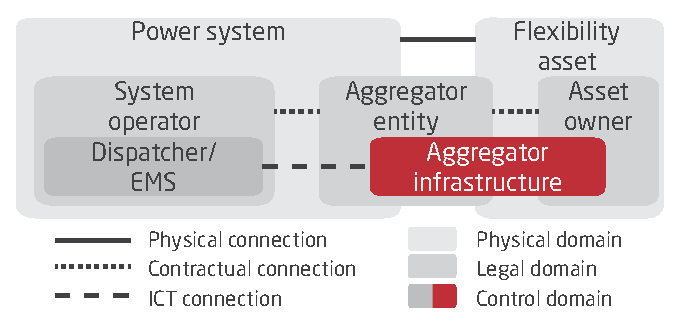
\includegraphics[width=1.0\columnwidth]{etfa2015/domains.eps}
\caption{The aggregator concept across domains.}
\label{fig:domains}
\vspace*{-5mm}
\end{figure}
\subsection{Clarifying the Aggregator concept}\label{subsec:clarifying}
The term \emph{aggregation} has different relevant interpretations in business, information technology,  control, as well as in the physical power system domain. Our concept of aggregators is illustrated in Fig.~\ref{fig:domains}, defining aggregators as a business role, aggregator entity, as well as a technical aggregator infrastructure.

The physical domain addresses the electrical interactions between flexibility assets (also referred to as DER) and power system. Whereas aggregation with respect to physical topology is a common concept (e.g. microgrids, cells), in our understanding, aggregators are not bound to aggregation with respect to physical network topology. 
%The aggregator is only reflected in this level by the manipulation of the interaction between the flexibility assets and the power system.

In the legal and business domain, an aggregator entity is an intermediary, maintaining contractual relations with flexibility asset owners and system operators (as receivers of flexibility services). The aggregator entity assumes legal responsibility for the delivery of a contracted service. The aggregator role may be filled by new independent market actors or be part of existing actors, such as utilities or balance responsible parties.

In the control domain, the aggregator infrastructure coordinates the behavior of flexibility assets. The control domain requirements are formulated as \emph{flexibility services} to system operators and \emph{asset management services} towards asset owners. Tracing these requirements for architectural validation and performance validation in the aggregator infrastructure is the focus of this paper.

The proposed aggregator concept is implementation agnostic and focused on formulation of functional requirements.

\subsection{The aggregator concept in technical literature}
There is no unanimous definition in literature of what could be considered standard functionality of an aggregator. This is reflected by the wide variety of aggregator designs\fcite{kok2005powermatcher,han2010development,sortomme2011optimal,costanzo2013coordination}, which differ in capabilities and purpose, and which use different (often implicit) criteria for classification.

Aggregators are commonly classified by control scheme into autonomous, indirect, transactional and direct control \fcite{Kosek}. Another classification emphasizes the commercial or technical focus of aggregators, referring to \emph{commercial} and \emph{technical} virtual power plants (CVPP and TVPP) \fcite{fenix2009}; however, as both types require business and technical functionality, the CVPP/TVPP distinction expresses a difference in degree and is not categorical. An advanced aggregator realizing the full functionality spectrum as \emph{Dynamic VPP} (DVPP) has been formulated in other work\fcite{niesse2014conjoint}. 
The proposed concept of aggregation encompasses all of the above but focuses on functional requirements for service provision, not business logic.

\subsection{Aggregator Business Harmonization and Standardization}
Whereas aggregator functionality is becoming a shared concept, there are still many models describing a) which stakeholders may benefit from the flexibility service, b) the form of the flexibility service, c) which stakeholders (are allowed to) perform aggregation and who should receive compensation \fcite{eurel-aggr} and d) how to harmonize the interaction between aggregators and aggregated units.

With respect to a), market models are being revised and new service models introduced to assign a value to flexibility (either directly to system operators as ancillary service, or as enhancement of flexibility of existing portfolios). The form of the service, b), is often formulated as an abstract flexibility service, a trade-off between both grid needs and generalized resource characteristics. Regarding d), many aggregators use proprietary communication, loosely based on standards (e.g. IEC61850 or IEC 60870-5-104; increasingly also OPC-UA); harmonization efforts in Europe continue to be addressed in the Smart Grid Coordination Group (SGCG) under EU Mandate M/490. A successful interoperability effort in this domain is the OpenADR standard published also as IEC PAS 62746.10-1. Meanwhile the IEC TR 62357 \emph{Reference Architecture to Smart Grid Information Exchange} is under revision. The reference architecture presented here focuses, within the Smart Grid Architecture Model\fcite{SGAM}, on functional interoperability for aggregators (field to operation zones; DER and customer domains) supporting interactions with System Operators, market actors, and devices at process level.

%\noindent\rule{4cm}{0.4pt}\\
%\textcolor{red}{(the follwoing defintioins belong into this section)}\\
%DEFINITION\\
%LEGAL\\
%Aggregator Role $\surd$\\
%Flexibility Asset Owner Role $\surd$\\
%SOFTWARE DOMAIN\\
%Virtual Nodes  (agents, processes) $\surd$ \\
%aggregator-side $\surd$ \\
%asset-side $\surd$ \\
%PHYSICAL DOMAIN \\
%Aggregator Site\\
%Flexibility Asset $\surd$ \\
%Device Interface $\surd$ \\ 

%#############################################
\section{The Need for an Aggregator Reference Architecture}
\label{sec:requirements}
%The power system is experiencing a paradigm shift. 
Existing concepts and methods for benchmarking and generator validation/certification cannot readily be translated from the (bulk) generator based paradigm to the distributed paradigm of aggregators and flexibility services. Historically, ancillary services have been defined using a physical understanding of generator capabilities. This definition is moving towards technology-agnostic service models.
Service verification has been done through on-site measurements, which is infeasible with thousands of units participating in service provision.  

The definition of a reference architecture for aggregators addresses these three issues, and enables benchmarking of aggregator architectures.
A reference architecture ``captures the essence of existing architectures, and the vision of the future needs and evolution to provide guidance to assist in developing new system architectures.''\cite{cloutier2010concept}. It should provide: 
\begin{itemize}
\item a common lexicon and taxonomy,
\item modularization and the complementary context, and
\item a common (architectural) vision.
\end{itemize} 

%1) new industry -> benchmark, kpis certification is needed, since they cannot be translated from the old industry 
%
%2) service verification is different -> traditionally expensive measuring equipment. new method is needed for new architecture
%
%3) technology agnostic service models, rather than technology based services. Need an architecture to standardize context
%The common lexicon and taxonomy allows for precise discussion and a common understanding of what an aggregator is and can do. The establishment of these two concepts is started in Section~\ref{subsec:clarifying}, where the context of the aggregator is also discussed.% and further refined throughout the paper. 
Various types of aggregator implementation exist, realizing different design ideas for different sets of requirements. These requirements -- and consequently the designs derived from them -- are unlikely to converge towards a single solution because of the tradeoffs involved, e.g. scalability and complexity. A common lexicon and taxonomy is a minimal precondition for aggregator comparison.
If a reference architecture is to be used to describe many of these different designs, it must be highly modular. In practice, the \emph{general} functionality of an aggregator must be broken down into small enough functions in order for these functions to be usable as building blocks for the reconstruction of the \emph{particular} functionality of a given implementation. 
The functions are arranged in a reference architecture such that metrics can be assigned to individual functions. In this way, the reference architecture can be used for validation of the aggregator. Our architectural vision accounts for the need for verifying distributed flexibility services.

%Implementability (discuss what that means in this context?)

%The methodology for the analysis is the following:
%\begin{itemize}
%	\item We have analyzed different aggregator architectures from the literature, as well as the experience gained through the practical implementation of an aggregator in our laboratory, and extracted the essential functionalities necessary for the working of the aggregator. These functionalities are independent from aggregator/control architecture.
%	\item We analyze the functions and their relationships, as well as the level of complexity we can foresee.
%	\item Synthetize the results into a reference architecture. 
%	\item Validate by mapping different architectures into the framework.
%\end{itemize}


%This is still part state of the art, so this and the previous section together shouldn't be too long)
%\begin{itemize}
%\item \textit{The method}
%\item Why would somebody want to evaluate aggregator performance?
%\item Which methods/approaches for performance evaluation exist or are being discussed?
%\item What is missing? (A reference architecture of course, but why?)
%\end{itemize}

%#############################################
\section{Functional decomposition}
\label{sec:funcdec}
An aggregator is a complex system of interacting functions. In the following definitions, we abstract from implementation details, e.g. centralized vs. distributed systems, and focus purely on the purpose of the functions. 

% EXTERNAL INTERFACES
%\subsection{Service Interface}
\textbf{A. Service Interface}
The service interface translates the contractual agreements between the aggregator and its clients into a service model containing quantifiable and measurable service requirements and a set of performance criteria. This service model is then used to map incoming service requests to control domain signals such as control variables, constraints or control parameters.


% Monitoring & Supervision modules
%\subsection{Performance Monitoring}
\textbf{B. Performance Monitoring}
The performance monitoring function collects data from which the behaviour of individual clients can be derived. The data is analyzed to determine the performance of a client, and its compliance with the contracted flexibility service. This analysis may be internal to the performance monitoring function, or it may simply serve as a data gatherer for an external entity.


%\subsection{Supervision and Resource Handling}
\textbf{C. Supervision and Resource Handling}
The aggregator must maintain an overview of available client resources and their status. By comparing the communication status and monitored performance of individual clients to the control signals sent by the aggregator, the supervision function determines whether clients perform according to their contract. It may temporarily or permanently exclude non-compliant clients from the pool of available resources.


%\subsection{Operator Interface}
\textbf{D. Operator Interface}
Although the power system is moving towards automated solutions, decision-making on critical issues is the responsibility of human operators. The aggregator architecture must support decision-making by presenting operators with the necessary information, and facilitating operator input and intervention.  %\textcolor{red}{(Incomplete/rewrite!)}


% Control-related
%\subsection{Control}
\textbf{E. Control}
The control function is in charge of generating the appropriate control domain signals for the portfolio. Depending on the control architecture, the control logic may be distributed between physical entities. The concept of a control domain signal covers several kinds of signals, including, but not limited to control inputs to DERs, coordination messages for distributed control and reference signals for hierarchical controllers.


%\subsection{Flexibility Monitoring}
\textbf{F. Flexibility Monitoring}
In operation, the aggregator must assess the future flexibility of its portfolio in real time; this includes individual DER flexibility as well as the aggregated flexibility of the portfolio. The flexibility assessment can either be based on direct feedback from the DERs or entirely on estimation models (possibly stochastic) if direct feedback is not available.

% Communication
%\subsection{Aggregator-internal communication}
\textbf{G. Aggregator-internal communication}
Except for very few special cases, aggregation will almost always be implemented as a distributed computing system. In its basic form, such a system would consist of one aggregator and a number of clients. This may be extended by stacking multiple levels of aggregation etc. The internal communication function exchanges information between aggregator and clients.


%\subsection{Client management}
\textbf{H. Client management}
The client management function actively or passively tracks the availability of clients. It may also provide a mechanism for the dynamic addition and removal of clients, such as a discovery service, and maintain a protocol for temporarily disabling otherwise available resources. It contributes to resilience and graceful degradation of the portfolio.



%\subsection{External Information Services}
\textbf{I. External Information Services}
To be able to act optimally with respect to both control of its portfolio and trade of electricity in forward markets, aggregators will likely have to rely on different types of information services. Such services include different types of forecasts and measurements in real time and may be provided by either internal processes or by a 3rd party. 


%\subsection{Asset interface}
\textbf{J. Asset interface}
Most aggregators in a Smart Grid context will be used to harvest flexibility from existing energy resources. In most cases communication between aggregator and resource will use a fieldbus-style interface not designed for wide-area communication. The purpose of the asset interface is to maintain communication with a physical unit under aggregator control and provide abstraction from interface details.


% the odd one
%\subsection{Information Exchange}
\textbf{K. Information Exchange}
Virtually any modular software framework contains a facility for information exchange between its components and storage of the overall system state: static data, dynamic data or both. A knowledge exchange may take many different forms, from a collection of object references towards a central or distributed database. 


%#############################################
\section{The Reference Architecture} 
\label{sec:refarch}
% === This is where we collect the knowledge collected in the previous section into the actual architecture and discuss it and its building blocks. (Introduce complexity levels) ===

We have now established a set of functions to serve as building blocks for a reference architecture, but without concern for the relations between these blocks. Next, these relations will be examined; in other words: how could a practical aggregator infrastructure be composed from these function blocks?

\subsection{Function blocks and knowledge exchange diagram}

% === Explain what the function blocks symbolize - and how the location in the function block diagram does not say anything about whether a block exists on the aggregator side, the client side or both. ===

The functions in section \ref{sec:funcdec} generally belong to one of the following categories:
\begin{itemize}
\item functions dedicated to communication between physically separate parts of the aggregator infrastructure or communication with 3rd party entities, i.e. enablers of the distributed nature of the system.
\item functions which perform decisions with regards to flexibility asset behavior and portfolio composition.
\item functions which interpret information and support the decision making functions. 
\end{itemize}
These categories represent requirements for different architectural paradigms: Communication functions are layered or hierarchical, and, in the case of communication between aggregator and client, require an identically layered counterpart at the opposite end. The decision making and interpreter functions on the other hand require many hierarchical and non-hierarchical consumer-producer relations. % The interpreter functions generally exist in direct relationship with the decision making functions. %The knowledge exchange function, storing the different elements of system state, provides a link between these two worlds.  
Figure~\ref{fig:functiondiagram} shows an overview of the relationships between functions according to the above concept.

\begin{figure}[htb]
\centering
\includegraphics[width=1.0\columnwidth]{"figures/diag_simple"}
\caption{Each function outputs distinct kinds of data which are used by the other functions in different ways according to the aggregator implementation.}
\label{fig:functiondiagram}
\end{figure}

\subsection{Principles of distribution of functions}

While figure \ref{fig:functiondiagram} depicts the relationship between aggregator functions, it does not include information about the physical distribution of these functions between the asset side and the operator side of the aggregator infrastructure. This distribution is highly specific to the individual design and e.g. its degree of centralization (see section \ref{sec:applic}).

In an actual implementation, several of these functions require corresponding instances on each side, effectively forming a communication stack. 

The functions exhibiting these properties are:
\begin{itemize}
\item the internal aggregator communication function which provides the link between the two substacks. In many cases, this function will make use of a full OSI-layered stack in which the internal aggregator communication function provides the application layer,
\item the client management function, implementing management protocols which would typically require a corresponding instance on the client side, and
\item the knowledge exchange function which exchanges information with its client side counterpart independent of client management mechanisms.
\end{itemize}

All other functions, with the exception of the asset interface, may appear either on the operator side, on the asset side, or shared between both sides, depending on the implementation.

%#############################################
\section{Case studies} 
\label{sec:applic}

A number of existing aggregator designs -- commercial as well as academic -- have been mapped to the model in order to test its viability. Two cases with different design philosophies are presented here in order to illustrate the distribution of functionality between the operator and the asset side, and the information flow between the functions:
\begin{itemize}
\item \emph{Power Hub} is an aggregator developed by Dong Energy in Denmark. It is used to control distributed generation and load in order to sell flexibility services to the ancillary power market (Figure~\ref{fig:powerhub}).
\item \emph{Open Energi} is a British company selling flexible consumption from industrial loads as an ancillary service. The aggregator functions are distributed between an operator node at a control center and asset nodes on custom hardware deployed at customer sites (Figure~\ref{fig:openenergi}).
\end{itemize}

The most significant difference between the two designs is the degree of autonomy of the asset node. The Power Hub concept is based on a centralized design which mainly uses the asset node as a communication gateway and places flexibility monitoring and control at the central operator site. This is also where external information such as market data is available through the information services function.
The Open Energi controller acts on quantities measurable at the asset site and does not require external information; this allows control and flexibility monitoring to be placed at the asset node, leaving only supervisory functions at the operator site.

Both designs can be split into functions according to the subdivision proposed in section \ref{sec:funcdec}.

\begin{figure}[htb]
\centering
\includegraphics[width=0.65\columnwidth]{"figures/stackdrawing_powerhub"}
\caption{Distribution of functions for the Power Hub aggregator}
\label{fig:powerhub}
\vspace*{-5mm}
\end{figure}
\begin{figure}[htb]
\centering
\includegraphics[width=0.65\columnwidth]{"figures/stackdrawing_openenergi"}
\caption{Distribution of functions for the Open Energi aggregator}
\label{fig:openenergi}
\vspace*{-5mm}
\end{figure}



%#############################################
\section{Conclusion and further work}
\label{sec:conclusion}
A reference architecture for the validation and comparison of aggregators has been presented. While the general framework has been established and successful mapping tests to a number of real-world aggregator designs have been performed, many details are still work in progress.
The next steps towards completion will be the development of performance indicators for the individual functions and the establishment of a process for aggregator comparison and performance validation.

%Review 1: As the goal of the paper is to develop a reference architecture, please elaborate on reference architectures in general and on the SGAM in particular.

%
%Review 2: The WIP-paper presents a high-level reference architecture for the validation and comparison of aggregators for power system services from distributed energy resources. Based on a functional decomposition of practical implementations a reference architecture is developed. It is validated against two practical implementations (power hub and open energi). 
%
%The value of a reference architecture for the crucial role of aggregators such as this is obvious but the developed architecture needs to be validated with more practical examples. How and if this architecture may be used performance evaluation, comparison or even optimization of aggregators remains to be proven. But the paper definitely meets the requirements of a WIP contribution.

%Review 3:	The concept of the reference architecture is nicely introduced and explained. Since it is a work in progress paper a more detailed presentation of future work would be appreciated.

% An example of a floating figure using the graphicx package.
% Note that \label must occur AFTER (or within) \caption.
% For figures, \caption should occur after the \includegraphics.
% Note that IEEEtran v1.7 and later has special internal code that
% is designed to preserve the operation of \label within \caption
% even when the captionsoff option is in effect. However, because
% of issues like this, it may be the safest practice to put all your
% \label just after \caption rather than within \caption{}.
%
% Reminder: the "draftcls" or "draftclsnofoot", not "draft", class
% option should be used if it is desired that the figures are to be
% displayed while in draft mode.
%
%\begin{figure}[!t]
%\centering
%\includegraphics[width=2.5in]{myfigure}
% where an .eps filename suffix will be assumed under latex, 
% and a .pdf suffix will be assumed for pdflatex; or what has been declared
% via \DeclareGraphicsExtensions.
%\caption{Simulation Results.}
%\label{fig_sim}
%\end{figure}

% Note that IEEE typically puts floats only at the top, even when this
% results in a large percentage of a column being occupied by floats.


% An example of a double column floating figure using two subfigures.
% (The subfig.sty package must be loaded for this to work.)
% The subfigure \label commands are set within each subfloat command,
% and the \label for the overall figure must come after \caption.
% \hfil is used as a separator to get equal spacing.
% Watch out that the combined width of all the subfigures on a 
% line do not exceed the text width or a line break will occur.
%
%\begin{figure*}[!t]
%\centering
%\subfloat[Case I]{\includegraphics[width=2.5in]{box}%
%\label{fig_first_case}}
%\hfil
%\subfloat[Case II]{\includegraphics[width=2.5in]{box}%
%\label{fig_second_case}}
%\caption{Simulation results.}
%\label{fig_sim}
%\end{figure*}
%
% Note that often IEEE papers with subfigures do not employ subfigure
% captions (using the optional argument to \subfloat[]), but instead will
% reference/describe all of them (a), (b), etc., within the main caption.


% An example of a floating table. Note that, for IEEE style tables, the 
% \caption command should come BEFORE the table. Table text will default to
% \footnotesize as IEEE normally uses this smaller font for tables.
% The \label must come after \caption as always.
%
%\begin{table}[!t]
%% increase table row spacing, adjust to taste
%\renewcommand{\arraystretch}{1.3}
% if using array.sty, it might be a good idea to tweak the value of
% \extrarowheight as needed to properly center the text within the cells
%\caption{An Example of a Table}
%\label{table_example}
%\centering
%% Some packages, such as MDW tools, offer better commands for making tables
%% than the plain LaTeX2e tabular which is used here.
%\begin{tabular}{|c||c|}
%\hline
%One & Two\\
%\hline
%Three & Four\\
%\hline
%\end{tabular}
%\end{table}


% Note that IEEE does not put floats in the very first column - or typically
% anywhere on the first page for that matter. Also, in-text middle ("here")
% positioning is not used. Most IEEE journals use top floats exclusively.
% Note that, LaTeX2e, unlike IEEE journals, places footnotes above bottom
% floats. This can be corrected via the \fnbelowfloat command of the
% stfloats package.


%#############################################
\section*{Acknowledgment}
Parts of this work are supported by the Programme for Energy Technology Development and Demonstration (EUDP) and Innovation Fund Denmark through the iPower project.

% Can use something like this to put references on a page
% by themselves when using endfloat and the captionsoff option.
\ifCLASSOPTIONcaptionsoff
  \newpage
\fi



% trigger a \newpage just before the given reference
% number - used to balance the columns on the last page
% adjust value as needed - may need to be readjusted if
% the document is modified later
%\IEEEtriggeratref{8}
% The "triggered" command can be changed if desired:
%\IEEEtriggercmd{\enlargethispage{-5in}}

% references section

% can use a bibliography generated by BibTeX as a .bbl file
% BibTeX documentation can be easily obtained at:
% http://www.ctan.org/tex-archive/biblio/bibtex/contrib/doc/
% The IEEEtran BibTeX style support page is at:
% http://www.michaelshell.org/tex/ieeetran/bibtex/
\bibliographystyle{IEEEtran}
% argument is your BibTeX string definitions and bibliography database(s)
\bibliography{bib/IEEEabrv,bib/references}
%
% <OR> manually copy in the resultant .bbl file
% set second argument of \begin to the number of references
% (used to reserve space for the reference number labels box)

% biography section
% 
% If you have an EPS/PDF photo (graphicx package needed) extra braces are
% needed around the contents of the optional argument to biography to prevent
% the LaTeX parser from getting confused when it sees the complicated
% \includegraphics command within an optional argument. (You could create
% your own custom macro containing the \includegraphics command to make things
% simpler here.)
%\begin{IEEEbiography}[{\includegraphics[width=1in,height=1.25in,clip,keepaspectratio]{mshell}}]{Michael Shell}
% or if you just want to reserve a space for a photo:



% You can push biographies down or up by placing
% a \vfill before or after them. The appropriate
% use of \vfill depends on what kind of text is
% on the last page and whether or not the columns
% are being equalized.

%\vfill

% Can be used to pull up biographies so that the bottom of the last one
% is flush with the other column.
%\enlargethispage{-5in}



% that's all folks
\end{document}


